\documentclass{beamer}

\usetheme{Madrid}
\setbeamertemplate{navigation symbols}{}

\usepackage{graphicx}
\DeclareGraphicsExtensions{.pdf,.png,.jpg}
\graphicspath{ {./img/} }

\usepackage{amsmath}
\usepackage{mathtools}

\title[Features]{Comparison of different Features Detectors and Descriptors in the Cut-Copy Forgery scenario}
\institute[CSI 445]{
    CSI 445 - Digital Image Forensics
}
\author[Seraphini,Teixeira]{Sibelius Seraphini, Larissa Teixeira}
\date{}

%\usetheme{Warsaw}

\begin{document}

    \frame{\titlepage}

    \begin{frame}
        \frametitle{Introduction}
        \begin{itemize}[<+->]
            \item Social Media (Twitter, Facebook, Youtube, and the blogosphere)
            
\includegraphics[width=10cm]{social_media}
        \end{itemize}
    \end{frame}

%Precision: 0.98 (+/- 0.01)
%Recall: 0.98 (+/- 0.01)
%F1 Score: 0.98 (+/- 0.00)

    \begin{frame}
        \frametitle{Motivation}
        \begin{itemize}
            \item Can we extract crime information from the social media?
        \end{itemize}
    \end{frame}

    \begin{frame}
        \frametitle{Applications}
        \begin{itemize} [<+->]
            \item Crowdsourcing crime visualization
                \begin{itemize}
                    \item Crime information from the social media
                    \item Crime information directly from the users
                \end{itemize}
            \item Safety Routing
                \begin{itemize}
                    \item Based on crime information provide a safety routing for one place to another
                \end{itemize}
            \item Crime Alert
                \begin{itemize}
                    \item Panic Button alerts a new crime based on GPS information
                    \item A espace safety route is provided to the user
                    \item The police can be notified
                \end{itemize}
        \end{itemize}
    \end{frame}

    \begin{frame}
        \frametitle{Social Media Crime Information Extraction}
        \begin{columns}[c]
            \column{3in}
            \begin{enumerate} [<+->]
                \item Crawl tweets from Twitter
                \item Classify tweets in related to crime or not
                \item Determine the type of crime
                \item Extract Location of tweet
            \end{enumerate}
        
            \column{1in}
            
\includegraphics[width=1in]{twitter}
        \end{columns}
        % More content goes here
        %\includegraphics[width=12cm]{application}
    \end{frame}

    \begin{frame}
        \frametitle{Crawl tweets from Twitter}
        \begin{itemize}
            \item Streaming API
                \begin{itemize}
                    \item New York city region
                    \item Keywords related to crime
                \end{itemize}
        \end{itemize}
    \end{frame}

    \begin{frame}
        \frametitle{Classification of tweets}
        \begin{itemize}
            \item<1-> Training Data
                \begin{itemize}
                    \item 14094 tweets manually labeled (5837 positives, 8257 negatives)
                    \item Types of Crimes:
                    \begin{itemize}
                        \item Robbery, Shooting, Theft, Assault
                        \item Burglary, Vandalism, Arson, Drug Possession
                    \end{itemize}
                \end{itemize}
            \item<2-> Classifier of crime related Statistics
                \begin{itemize}
                    \item Precision: 0.98 (+/- 0.01)
                    \item Recall: 0.98 (+/- 0.01)
                    \item F1 Score: 0.98 (+/- 0.00)
                \end{itemize}
            \item<3-> Classifier of type of crimes Statistics
                \begin{itemize}
                    \item Precision: 0.92 (+/- 0.01)
                    \item Recall: 0.93 (+/- 0.01) 
                    \item F1 Score: 0.93 (+/- 0.01)
                \end{itemize}
        \end{itemize}
    \end{frame}

    \begin{frame}
        \frametitle{Extract Location of Tweet's text}
        \begin{itemize}[<+->]
            \item Preprocessing
                \begin{itemize}
                    \item Lowercase
                    \item Remove punctuation
                    \item Apply alias dictionary
                \end{itemize}
            \item Match street addresses (Begin of address)
            \item Match state names (End of address)
        \end{itemize}
    \end{frame}
    
    \begin{frame}
        \frametitle{Web App Interface}
        \url{http://morning-oasis-6740.herokuapp.com}
        \centering
        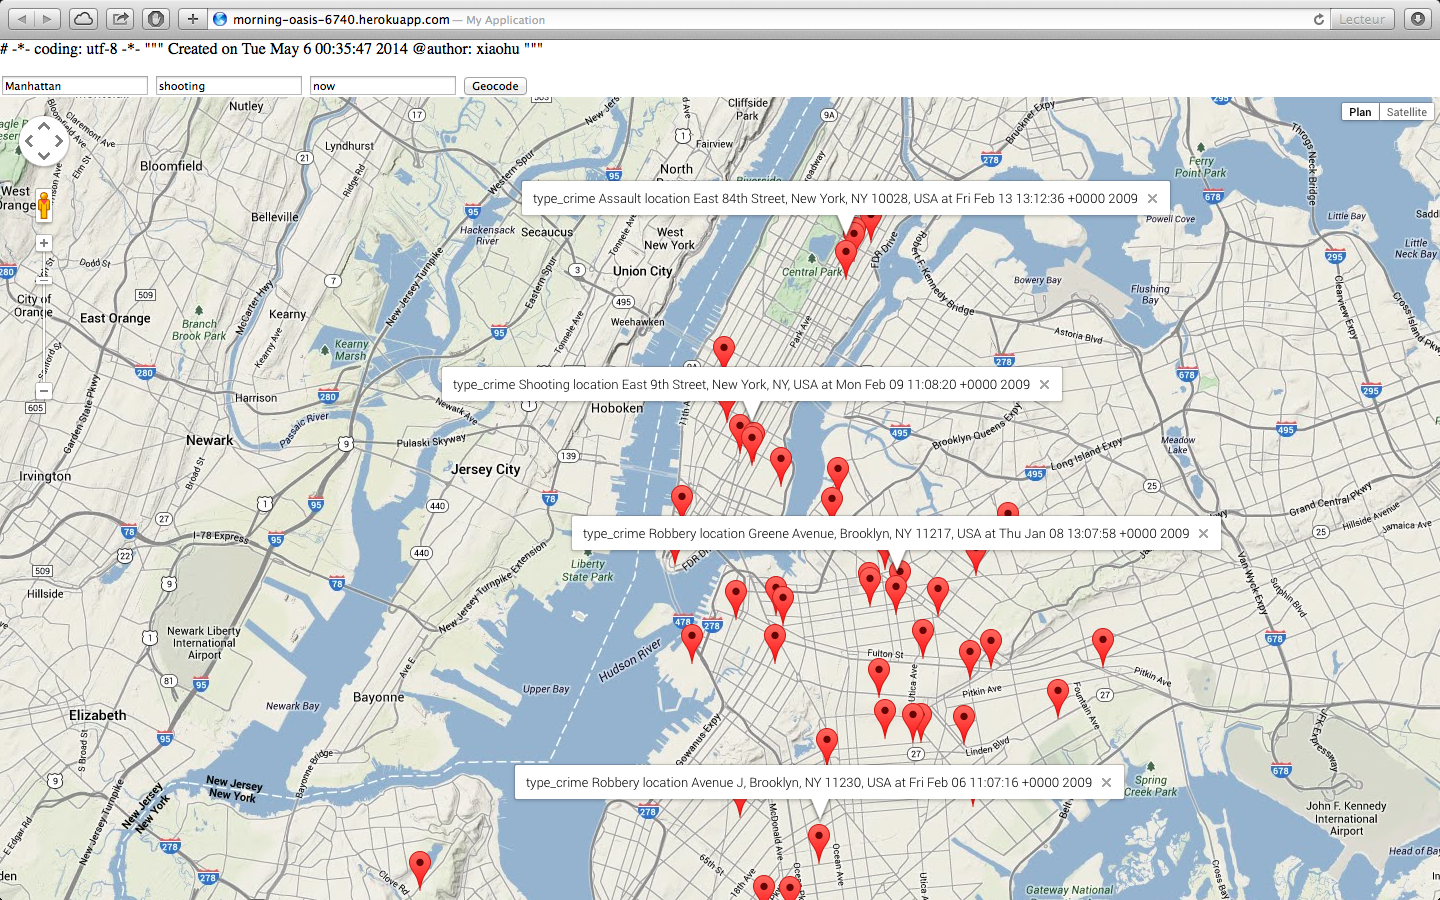
\includegraphics[width=12cm]{eagleeye_gui}
    \end{frame}
    
    \begin{frame}
        \frametitle{Questions ?}
        \centering
        
\includegraphics[height=9cm]{questions}
    \end{frame}

\end{document}
